\documentclass[letter,11pt]{article}

\usepackage[spanish,es-nodecimaldot]{babel}
\usepackage[utf8]{inputenc}

\usepackage{lmodern}
\usepackage[T1]{fontenc}
\usepackage{textcomp}

\usepackage{framed}
\usepackage[svgnames]{xcolor}

\usepackage{graphicx}
\usepackage{pstricks}

\usepackage{anysize}
\marginsize{3cm}{2cm}{2cm}{3cm}

\usepackage{siunitx}
\usepackage{amsmath}
\usepackage{array}

\usepackage{fancyhdr}
\usepackage{lastpage}
\pagestyle{fancy}
\fancyhf{}
\fancyhead[LE,RO]{Física Básica III}
\fancyfoot[CO,CE]{\thepage\ de \pageref{LastPage}}

\special{papersize=215.9mm,279.4mm}

\usepackage[
    pdfauthor={Carlos Eduardo Caballero Burgoa},%
    pdftitle={Física Básica III},%
    pdfsubject={1er Parcial},%
    colorlinks,%
    citecolor=black,%
    filecolor=black,%
    linkcolor=black,%
    urlcolor=black,
    breaklinks]{hyperref}
\usepackage{breakurl}

\newcommand{\blankpage}{
\newpage
\thispagestyle{empty}
\mbox{}
\newpage
}

\renewcommand{\arraystretch}{1.2}

\begin{document}

\begin{center}
    {\Large \bf{Primer parcial}}
\end{center}

\noindent\fbox{%
    \parbox{\textwidth}{%
        Estudiante: CABALLERO BURGOA, Carlos Eduardo \\
        Carrera: Ingeniería Electromecánica \\
        Correo: cijkb.j@gmail.com
    }%
}

\vspace{0.5cm}

\begin{enumerate}
\item En una mesa libre de fricción, se liberan una carga puntual de masa $m$ y
carga $Q$, y otra carga puntual también de masa $m$ pero carga igual a $2Q$. Si
la carga $Q$ tiene una aceleración inicial $A_0$, la aceleración de $2Q$ será:

\begin{itemize}
    \item \textcolor{blue}{$A_0$.} <- correcta?
    \item \textcolor{red}{$2\,A_0$.}
    \item $4\,A_0$.
    \item $A_0/2$.
    \item $A_0/4$.
\end{itemize}

\textbf{Solución:}

\begin{figure}[!h]
\centering
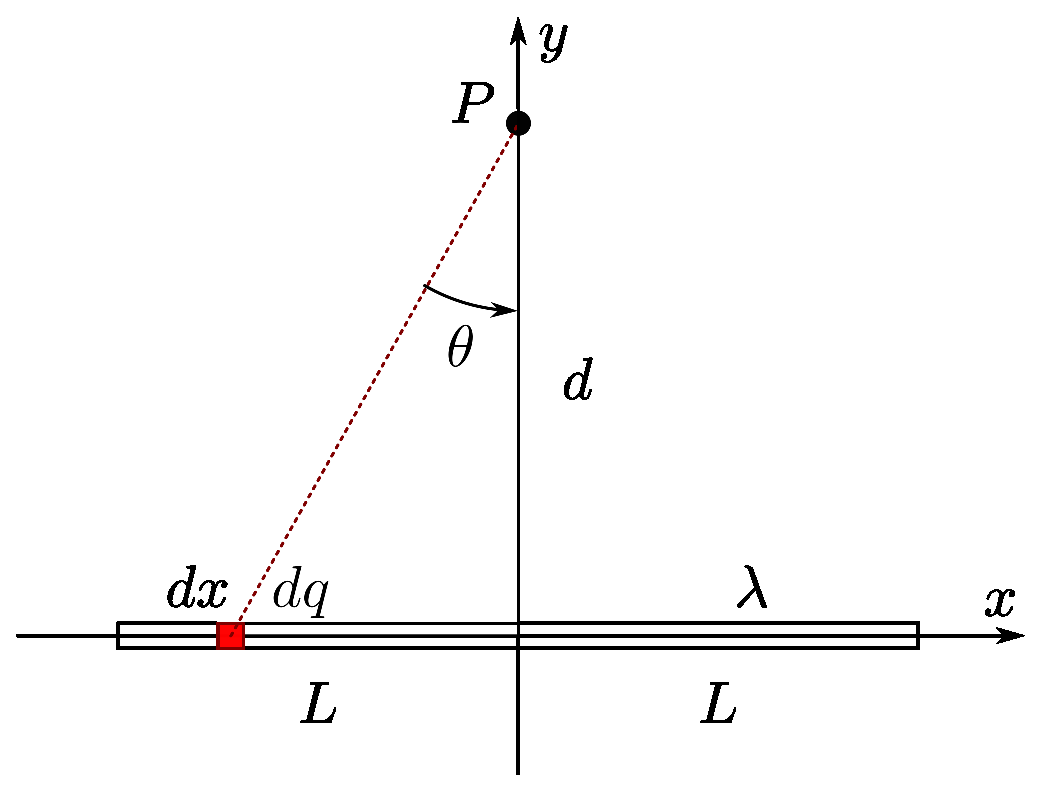
\includegraphics[scale=0.39]{resources/a1.eps}
\end{figure}

A partir del diagrama de cuerpo libre, sabemos:

\begin{equation*}
    \sum F_y = 0
\end{equation*}
\begin{equation*}
    \sum F_x = m\,a
\end{equation*}

Desarrollando $F_x$, y considerando que la aceleración $A_0$ es debido a un
campo eléctrico $E_x$:

\begin{equation*}
    E_x\,Q = m\,A_0
\end{equation*}
\begin{equation*}
    E_x = \frac{m}{Q}\,A_0
\end{equation*}

Considerando la segunda carga $2Q$:

\begin{equation*}
    E_x\,2Q = m\,A_1
\end{equation*}

Por tanto:

\begin{equation*}
    A_1 = E_x\,\frac{2Q}{m} = \frac{m}{Q}\,A_0 \frac{2Q}{m} = 2\,A_0
\end{equation*}

\item Usted tiene un anillo de oro puro con masa de $10.8 [g]$. El oro tiene una
masa atómica de $197 [g/mol]$ y un número atómico de $79$. Calcular la cantidad
de protones que tiene el anillo.

\begin{itemize}
    \item \num{8.54e24}.
    \item \num{4.27e24}.
    \item \num{3.41e22}.
    \item \num{5.64e22}.
\end{itemize}

\textbf{Solución:}

Haciendo las conversiones, obtenemos:

\begin{equation*}
    10.8 [g] \cdot
    \frac{1 [mol]}{197 [g]} \cdot
    \frac{\num{6.023e23}[átomo]}{1 [mol]} \cdot
    \frac{79 [protón]}{1 [átomo]} = \num{2.61e24}
\end{equation*}
\\

\item Dos esferas idénticas están atadas a cordones de seda de longitud
$L = 0.5 [m]$ y cuelgan de un punto común. Cada esfera tiene masa $m =8 [g]$. El
radio de cada esfera es muy pequeño por lo que pueden considerarse masas
puntuales. Se dan cargas positivas de magnitudes diferentes $Q_1$ y $Q_2$, lo
que hace que las esferas se separen, de manera que cuando están en equilibrio
cada cordón forma un ángulo de 20° con la vertical. Ahora se conecta un alambre
pequeño entre las esferas, lo cual permite que se transfiera carga de una a
otra, hasta que ambas esferas tengan la misma carga; entonces se quita el
alambre. Ahora cada cordón forma un ángulo de $30^\circ$ con la vertical.
Determine las cargas originales.

\begin{figure}[!h]
\centering
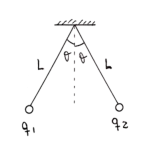
\includegraphics[scale=1.84]{resources/q3.eps}
\end{figure}

\begin{itemize}
    \item $\num{4.03e-6}[C]$ y $\num{2.21e-6}[C]$.
    \item $\num{1.81e-7}[C]$ y $\num{3.07e-7}[C]$.
    \item $\num{1.03e-7}[C]$ y $\num{2.23e-6}[C]$.
    \item \textcolor{red}{$\num{1.80e-7}[C]$ y $\num{2.06e-6}[C]$.} <- revisar
\end{itemize}

\textbf{Solución:}

\begin{figure}[!h]
\centering
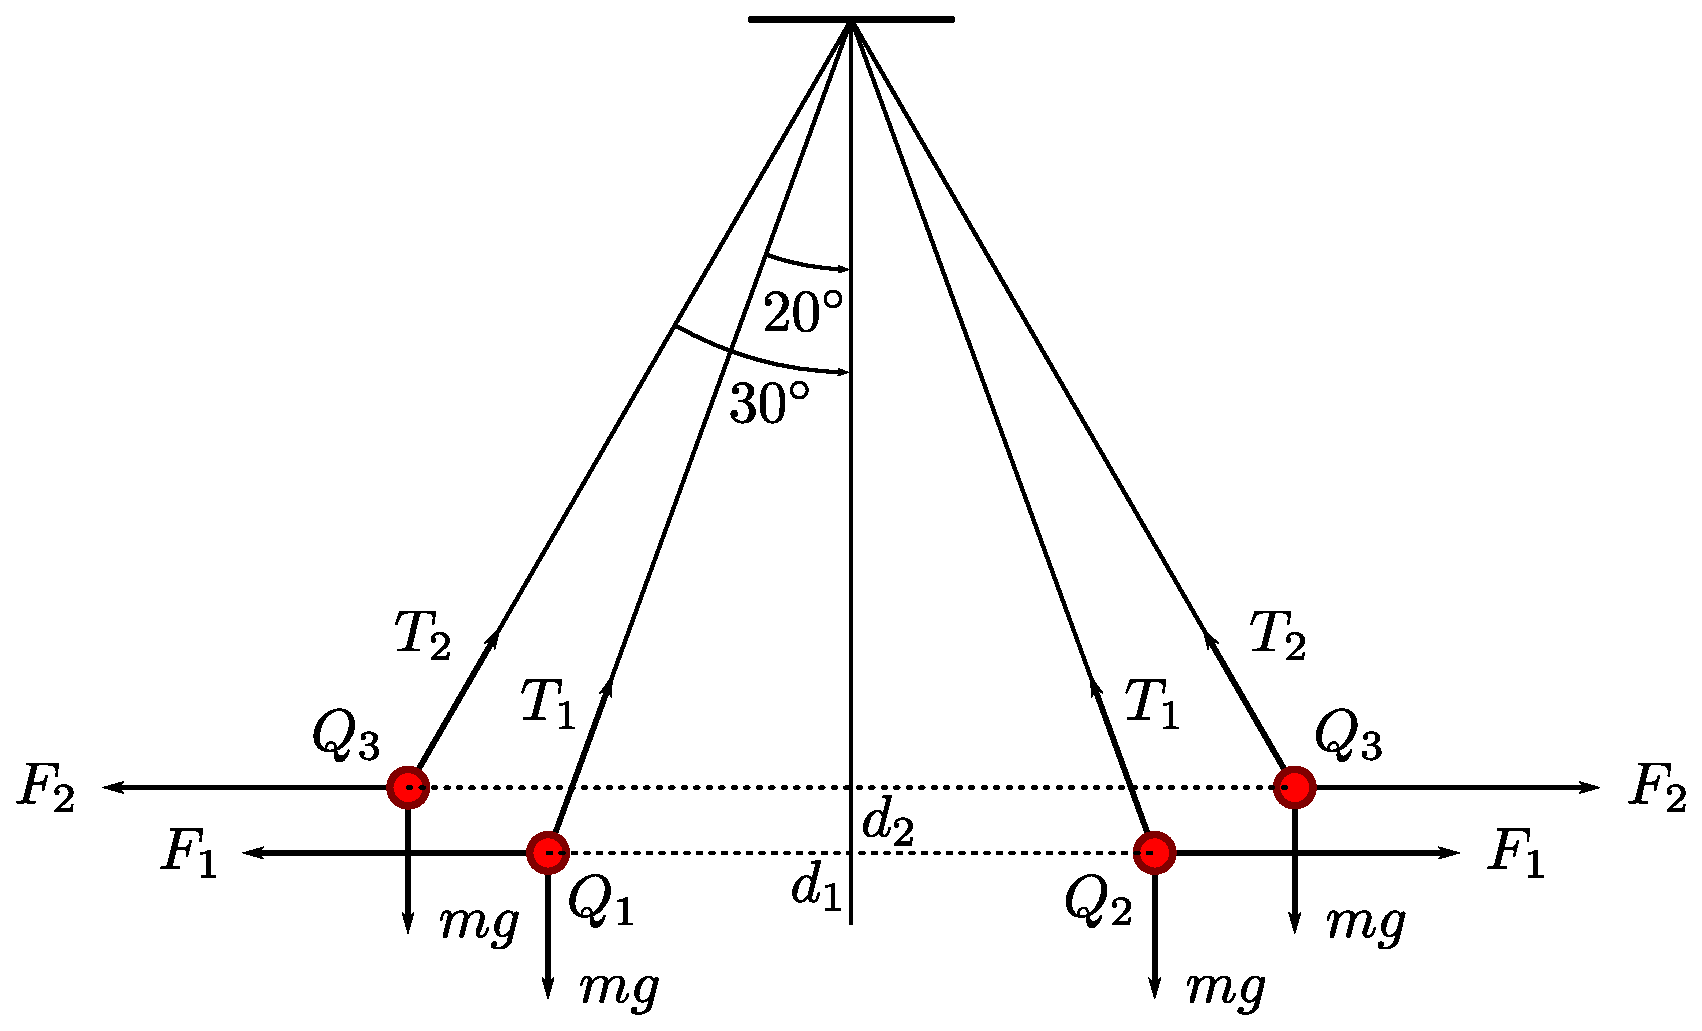
\includegraphics[scale=0.38]{resources/a3.eps}
\end{figure}

A partir del diagrama de cuerpo libre, sabemos:

\begin{equation*}
    \sum F_y = 0
\end{equation*}
\begin{equation*}
    \sum F_x = 0
\end{equation*}

Para el primer escenario:

\begin{equation*}
    \begin{cases}
        T_1\,cos(20^\circ)-mg = 0 \\
        T_1\,sen(20^\circ)-\dfrac{1}{4\pi\epsilon_0}\dfrac{Q_1\,Q_2}{d^2_1} = 0
    \end{cases}
\end{equation*}

Para el segundo escenario:

\begin{equation*}
    \begin{cases}
        T_2\,cos(30^\circ)-mg = 0 \\
        T_2\,sen(30^\circ)-\dfrac{1}{4\pi\epsilon_0}\dfrac{Q^2_3}{d^2_2} = 0 \\
        Q_1+Q_2 = 2\,Q_3
    \end{cases}
\end{equation*}

Para el calculo de $d^2_1$ y $d^2_2$, se usan la ley de cosenos:

\begin{equation*}
    d^2_1 = L^2+L^2-2(L)(L)\,cos(40^\circ)
\end{equation*}
\begin{equation*}
    d^2_1 = 2L^2\,(1-cos(40^\circ))
\end{equation*}
\begin{equation*}
    d^2_2 = 2L^2\,(1-cos(60^\circ))
\end{equation*}

Calculando $Q_3$:

\begin{equation*}
    T_2 = \frac{mg}{cos(30^\circ)}
\end{equation*}
\begin{equation*}
    \frac{mg}{cos(30^\circ)}\,sen(30^\circ) = \frac{1}{4\pi\epsilon_0}\frac{Q^2_3}{d^2_2}
\end{equation*}
\begin{equation*}
    Q^2_3 = mg\,tan(30^\circ)\,4\pi\epsilon_0\,d^2_2
\end{equation*}
\begin{equation*}
    Q^2_3 = mg\,tan(30^\circ)\,4\pi\epsilon_0\,2L^2\,(1-cos(60^\circ))
\end{equation*}
\begin{equation*}
    Q^2_3 = 8\pi\epsilon_0\,mg\,L^2\,tan(30^\circ)\,(1-cos(60^\circ))
\end{equation*}
\begin{equation*}
    Q^2_3 = \num{1.2599e-12}
\end{equation*}
\begin{equation*}
    Q_3 = \num{1.1225e-6} [C]
\end{equation*}

Calculando $Q_1\,Q_2$:

\begin{equation*}
    T_1 = \frac{mg}{cos(20^\circ)}
\end{equation*}
\begin{equation*}
    \frac{mg}{cos(20^\circ)}\,sen(20^\circ) = \frac{1}{4\pi\epsilon_0}\frac{Q_1\,Q_2}{d^2_1}
\end{equation*}
\begin{equation*}
    Q_1\,Q_2 = mg\,tan(20^\circ)\,4\pi\epsilon_0\,d^2_1
\end{equation*}
\begin{equation*}
    Q_1\,Q_2 = mg\,tan(20^\circ)\,4\pi\epsilon_0\,2L^2\,(1-cos(40^\circ))
\end{equation*}
\begin{equation*}
    Q_1\,Q_2 = 8\pi\epsilon_0\,mg\,L^2\,tan(20^\circ)\,(1-cos(40^\circ))
\end{equation*}

Considerando la conservación de la carga para calcular $Q_1$:

\begin{equation*}
    Q_2 = 2Q_3 - Q_1
\end{equation*}
\begin{equation*}
    Q_1\,(2Q_3 - Q_1) = 8\pi\epsilon_0\,mg\,L^2\,tan(20^\circ)\,(1-cos(40^\circ))
\end{equation*}
\begin{equation*}
    Q^2_1-2Q_3Q_1+8\pi\epsilon_0\,mg\,L^2\,tan(20^\circ)\,(1-cos(40^\circ))=0
\end{equation*}

Cuyas raíces son:

\begin{equation*}
    \begin{cases}
        Q1 = \num{2.0650e-06} [C] \\
        Q1 = \num{1.7998e-07} [C]
    \end{cases}
\end{equation*}

Para los cuales $Q_2$ son:

\begin{equation*}
    \begin{cases}
        Q2 = \num{1.7998e-07} [C] \\
        Q2 = \num{2.0650e-06} [C]
    \end{cases}
\end{equation*}
\\

\item Una línea larga tiene una densidad lineal de carga uniforme de
$\num{50e-6}[C/m]$ que es paralela y está a $10 [cm]$ de la superficie de una
lámina de plástico plana y grande que tiene una densidad superficial de carga
uniforme de $\num{-100e-6}[C/m2]$ en un lado. Encuentre la ubicación de una
carga puntual $Q$ donde la fuerza resultante sea cero debido a este arreglo de
objetos con carga.

\begin{itemize}
    \item $ 5.08 [cm]$ de la línea.
    \item $20.39 [cm]$ del plano.
    \item $10.22 [cm]$ de la línea.
    \item \textcolor{red}{$15.92 [cm]$ de la línea.}
\end{itemize}

\textbf{Solución:}

\begin{figure}[!h]
\centering
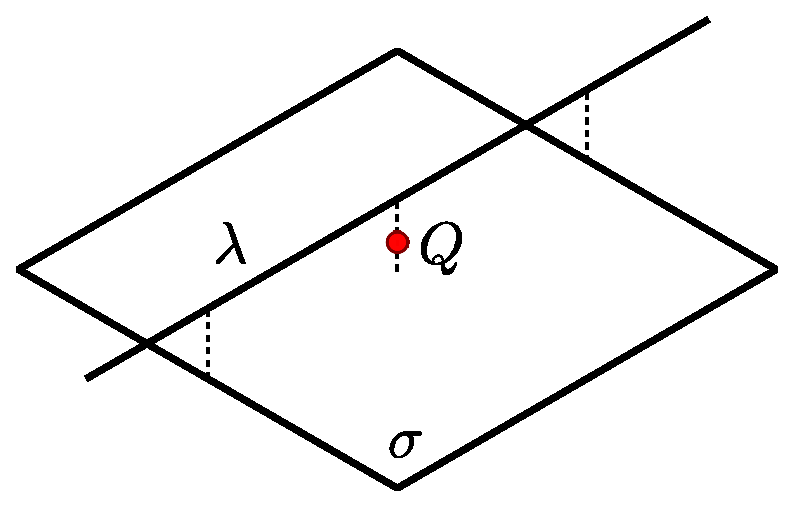
\includegraphics[scale=0.42]{resources/a4.eps}
\end{figure}

Sabiendo que el campo eléctrico de una linea continua es:

\begin{equation*}
    E_L = \frac{1}{2\pi\epsilon_0}\frac{\lambda}{r}
\end{equation*}

Y que el campo eléctrico de una superficie continua es:

\begin{equation*}
    E_S = \frac{\sigma}{2\epsilon_0}
\end{equation*}

Aplicando la condición de la carga puntual $Q$:

\begin{equation*}
    E_L - E_S = 0
\end{equation*}
\begin{equation*}
    \frac{1}{2\pi\epsilon_0}\frac{\lambda}{r}-\frac{\sigma}{2\epsilon_0} = 0
\end{equation*}
\begin{equation*}
    \frac{\lambda}{\pi\,r} = \sigma
\end{equation*}

Por tanto $r$ es:

\begin{equation*}
    r = \frac{\lambda}{\pi\,\sigma} = -0.1592 [m] = -15.92 [cm]
\end{equation*}
\\

\item Una carga $Q$ está distribuida uniformemente en el volumen de una esfera
aislante de radio $R = 4 [cm]$. A una distancia de $r = 8 [cm]$ desde el centro
de la esfera, el campo eléctrico debido a esta carga, tiene una magnitud de
$E = 940 [N/C]$. Calcular el campo eléctrico a una distancia de $2 [cm]$ del
centro de la esfera.

\begin{itemize}
    \item \textcolor{red}{$1880 [N/C]$.}
    \item $1760 [N/C]$.
    \item $2025 [N/C]$.
    \item $1539 [N/C]$.
\end{itemize}

\textbf{Solución:}

\begin{figure}[!h]
\centering
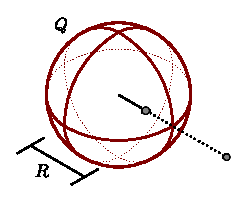
\includegraphics[scale=1.25]{resources/a5.eps}
\end{figure}

El campo eléctrico de una esfera aislante es:

\begin{equation*}
    E = \begin{cases}
        \dfrac{1}{4\pi\epsilon_0}\dfrac{Q}{r^2} & r > R \\
        \dfrac{1}{4\pi\epsilon_0}\dfrac{Q r}{R^3} & r < R
    \end{cases}
\end{equation*}

Se calcula la carga $Q$ a partir de la medición a $r = 8 [cm]$:

\begin{equation*}
    E = \frac{1}{4\pi\epsilon_0}\frac{Q}{r^2}
\end{equation*}
\begin{equation*}
    Q = 4\pi\epsilon_0\,E\,r^2 = \num{1.2112e-17} [C]
\end{equation*}

Con el valor de la carga $Q$, podemos calcular el campo eléctrico dentro la 
esfera:

\begin{equation*}
    E = \frac{1}{4\pi\epsilon_0}\frac{Q r}{R^3} =  1880 [N/C]
\end{equation*}
\\

\item Una carga puntual $Q_1 = 2.4 [\mu C]$ se mantiene estacionaria en el
origen. Una segunda carga puntual $Q_2 = -4.3 [\mu C]$ se mueve del punto
$x = 0.15 [m]$, $y = 0$ al punto $x = 0.25 [m]$, $y = 0.25 [m]$. Calcular el
trabajo que realiza la fuerza eléctrica sobre $Q_2$.

\begin{itemize}
    \item $ 0.265 [J]$.
    \item $-0.265 [J]$.
    \item $ 0.356 [J]$.
    \item \textcolor{red}{$-0.356 [J]$.}
\end{itemize}

\textbf{Solución:}

\begin{figure}[!h]
\centering
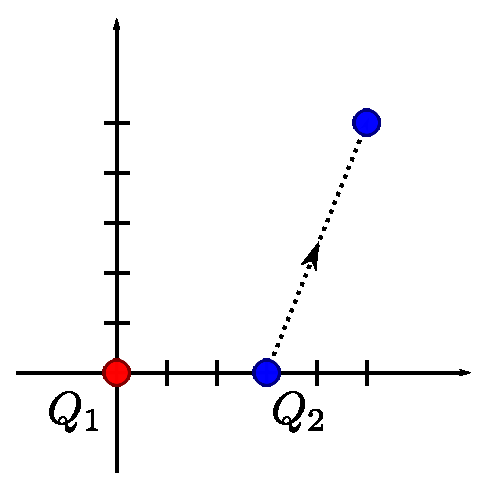
\includegraphics[scale=0.50]{resources/a6.eps}
\end{figure}

El trabajo $W$ sobre la carga $Q_2$ es:

\begin{equation*}
    W_{1 \rightarrow 2} = U_1 - U_2
\end{equation*}
\begin{equation*}
    W_{1 \rightarrow 2} = \frac{1}{4\pi\epsilon_0}\frac{Q_1Q_2}{r_1}-\frac{1}{4\pi\epsilon_0}\frac{Q_1Q_2}{r_2}
\end{equation*}
\begin{equation*}
    W_{1 \rightarrow 2} = \frac{Q_1Q_2}{4\pi\epsilon_0} \left(\frac{1}{r_1}-\frac{1}{r_2}\right) = -0.3560 [J]
\end{equation*}

\item Dos protones se liberan, a partir del reposo, cuando están separados
$0.75 [nm]$. Calcular la rapidez máxima que alcanzan.

\begin{itemize}
    \item \textcolor{red}{$13.56 [km/s]$.}
    \item $12.63 [km/s]$.
    \item $11.25 [km/s]$.
    \item $10.93 [km/s]$.
\end{itemize}

\textbf{Solución:}

\begin{figure}[!h]
\centering
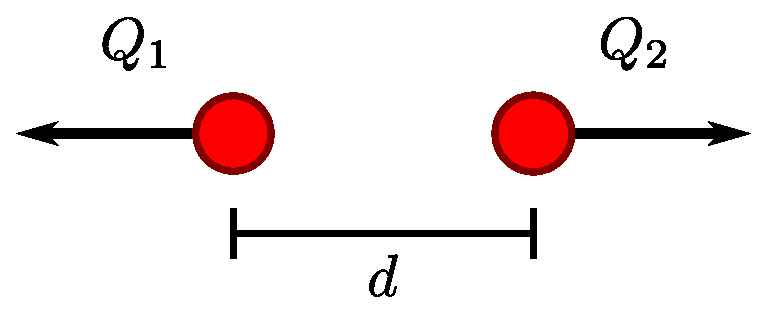
\includegraphics[scale=0.36]{resources/a7.eps}
\end{figure}

Considerando la conservación de la energía:

\begin{equation*}
    U_1+K_1 = U_2+K_2
\end{equation*}

Y sabiendo que cuando toda la energía potencial se ha convertido en energía
cinética, se da la velocidad máxima:

\begin{equation*}
    U_1 = K_2
\end{equation*}
\begin{equation*}
    \frac{1}{4\pi\epsilon_0}\frac{Q^2}{r} = \frac{1}{2}mv^2+\frac{1}{2}mv^2
\end{equation*}
\begin{equation*}
    v = \sqrt{\frac{1}{4\pi\epsilon_0}\frac{Q^2}{r}\frac{1}{m}} = \num{1.3554e4} [m/s] = 13.55 [km/s]
\end{equation*}
\\

\item Un cascarón cilíndrico aislante muy largo con radio de $6 [cm]$ tiene una
densidad de carga lineal de $\num{8.5e-6} [C/m]$ distribuida de manera uniforme
en su superficie exterior. Calcular la lectura de un voltímetro si se conectara
entre la superficie del cilindro y un punto a $4 [cm]$ por arriba de la
superficie.

\begin{itemize}
    \item $87.43 [kV]$.
    \item \textcolor{red}{$78.09 [kV]$.}
    \item $69.23 [kV]$.
    \item $55.66 [kV]$.
\end{itemize}

\textbf{Solución:}

\begin{figure}[!h]
\centering
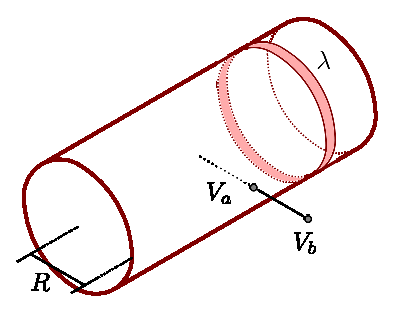
\includegraphics[scale=0.95]{resources/a8.eps}
\end{figure}

El campo eléctrico de un cascaron cilíndrico aislante es:

\begin{equation*}
    E = \begin{cases}
        \dfrac{1}{2\pi\epsilon_0}\dfrac{\lambda}{r} & r > R \\
        0 & r < R
    \end{cases}
\end{equation*}

Por tanto, el potencial eléctrico entre los puntos $a$ y $b$, es:

\begin{equation*}
    V_a-V_b = \int_{a}^{b}\vec{E}\cdot\vec{dl} = \int_{a}^{b}E_r\,dr = \int_{a}^{b}\frac{1}{2\pi\epsilon_0}\frac{\lambda}{r}dr
\end{equation*}
\begin{equation*}
    V_a-V_b = \frac{\lambda}{2\pi\epsilon_0}\int_{a}^{b} \frac{dr}{r} = \frac{\lambda}{2\pi\epsilon_0}\,ln (r)\Biggr|_{a}^{b} = \frac{\lambda}{2\pi\epsilon_0}(ln\,b-ln\,a)
\end{equation*}
\begin{equation*}
    V_a-V_b = \frac{\lambda}{2\pi\epsilon_0}\,ln\left(\frac{b}{a}\right) = 78048.2197 [V] = 78.05 [kV]
\end{equation*}
\\

\item Un capacitor cilíndrico consiste en un núcleo interior sólido de un
conductor con radio de $0.25 [cm]$, rodeado por un tubo conductor exterior
hueco. Los dos conductores están separados por aire, y la longitud del cilindro
es de $12 [cm]$. La capacitancia es de $36.7 [pF]$. Calcule el radio interior
del tubo hueco.

\begin{itemize}
    \item \textcolor{red}{$3 [mm]$.}
    \item $3.5 [mm]$.
    \item $4 [mm]$.
    \item $4.5 [mm]$.
\end{itemize}

\textbf{Solución:}

\begin{figure}[!h]
\centering
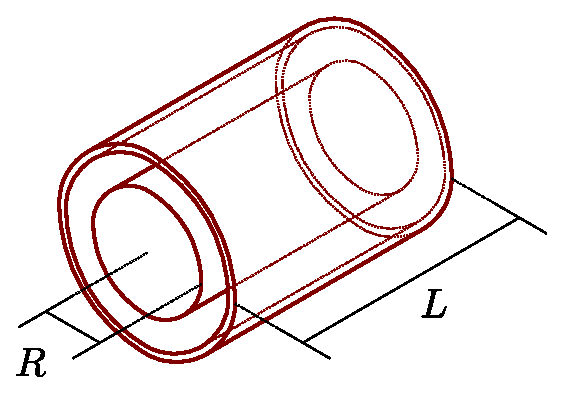
\includegraphics[scale=0.60]{resources/a9.eps}
\end{figure}

Se conoce que el potencial eléctrico de un cilindro es:

\begin{equation*}
    V_{ab} = \frac{\lambda}{2\pi\epsilon_0}\,ln\left(\frac{b}{a}\right)
\end{equation*}

Según la definición de capacitancia:

\begin{equation*}
    C = \frac{Q}{V_{ab}}
\end{equation*}

Y la definición de densidad lineal:

\begin{equation*}
    \lambda = \frac{Q}{L}
\end{equation*}

Se puede calcular el radio $r_b$:

\begin{equation*}
    V_{ab}\,C = Q
\end{equation*}
\begin{equation*}
    \frac{\lambda}{2\pi\epsilon_0}\,ln\left(\frac{r_b}{r_a}\right)\,C = \lambda\,L
\end{equation*}
\begin{equation*}
    ln\left(\frac{r_b}{r_a}\right) = 2\pi\epsilon_0\,\left(\frac{L}{C}\right)
\end{equation*}
\begin{equation*}
    r_b = r_a\,e^{2\pi\epsilon_0\,\left(\frac{L}{C}\right)} = \num{2.9987e-3} [m] = 2.9987 [mm]
\end{equation*}
\\

\item Un capacitor de $20 [\mu F]$ está cargado con una diferencia de potencial
de $800 [V]$. Las terminales del capacitor cargado se conectan entonces a las de
un capacitor descargado de $10 [\mu F]$. Calcule la energía total de esta nueva
configuración.

\begin{itemize}
    \item $6.45 [J]$.
    \item $5.27 [J]$.
    \item \textcolor{red}{$4.27 [J]$.}
    \item $3.33 [J]$.
\end{itemize}

\textbf{Solución:}

\begin{figure}[!h]
\centering
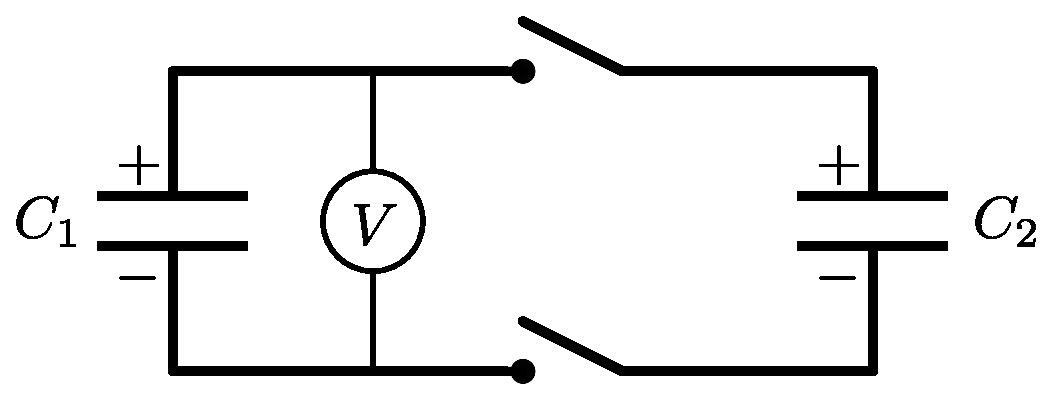
\includegraphics[scale=0.38]{resources/a10.eps}
\end{figure}

Se calcula la carga $Q_0$ del primer escenario:

\begin{equation*}
    C_1 = \frac{Q_0}{V_0}
\end{equation*}
\begin{equation*}
    Q_0 = C_1\,V_0 = 0,016 [C]
\end{equation*}

Al conectarse los dos capacitores, la carga $Q_0$ se conserva:

\begin{equation*}
    C_1+C_2 = \frac{Q_0}{V_1}
\end{equation*}
\begin{equation*}
    V_1 = \frac{Q_0}{C_1+C_2} = 533.33 [V]
\end{equation*}

La energía total es la suma de la energía en cada capacitor:

\begin{equation*}
    U_T = U_1+U_2 = \frac{1}{2}C_1\,V^2_1+\frac{1}{2}C_2\,V^2_1 = 4.2667 [J]
\end{equation*}

\end{enumerate}
\end{document}

